\section{Background}
\label{sec:background}

\subsection{\sotopia environment}
\label{sec:background:sotopia}
In this paper, we build on the \sotopia \citep{zhou2023sotopia} environment, introduced to evaluate language agents. \sotopia consists of \textit{social tasks}, where each task includes a scenario that provides information about the general setting, along with profiles of two characters and their respective goals, which are kept private from the other character. These combinations of scenarios and social goals are designed to cover a wide range of social interactions, such as collaboration, accommodation, and persuasion. For each social task, \sotopia prompts two large language models (LLMs) to act as role-playing \textit{social agents}, interacting with one another through \textit{speech, non-verbal communication, and actions.}

Consider an example as shown in Figure \ref{fig:sotopia}. The entire interaction between the two role-playing characters is called an \textit{episode} within \sotopia. Each episode consists of multiple turns. At each turn, the characters make decisions based on the context of the interaction, which includes (a) the scenario, (b) the character profile, (c) their private goal in the scenario, and (d) conversation history up to that point. The decision itself consists of two parts: (1) the action type, which can either be opting to \textit{speak} an utterance, perform a physical \textit{action}, engage in \textit{non-verbal communication} such as making a gesture, or \textit{leave} the conversation; (2) the content of the action type, which can be a string as an utterance (e.g., \emph{I have been feeling lonely lately'}), a physical action (e.g., \emph{switch car seats'}), or a non-verbal communication (e.g., \emph{`nodding your head'}). Leaving the conversation means exiting the episode.

In the paper, the authors also come up with an evaluation criteria, \sotopiaeval, where they list down seven social dimensions for evaluating the social intelligence of the role-playing characters. These dimensions include: goal completion (\goalcompletion), believability (\believability), knowledge (\knowledge), secret (\secret), relationship (\relationship), social rules (\socialrules) and financial and material benefits (\financialbenefits). In our paper, we only focus on the \goalcompletion and \believability dimensions for the evaluation of the language models (\S \ref{sec:framework:evaluation}). Each dimension is rated by GPT-4 \citep{openai2024gpt4} and humans on a Likert scale. The scores of different dimensions have three types of range: $[0,10]$, $[-10,0]$ and $[-5,5]$. The paper shows that when evaluating language models with \sotopiaeval, GPT-4 could serve as a proxy of human judgment on these dimensions, and it has a higher correlation and significance than human evaluations. Thus we also utilise GPT-4 as our primary evaluator for all the experiments.
\begin{figure}[!t]
    \centering
    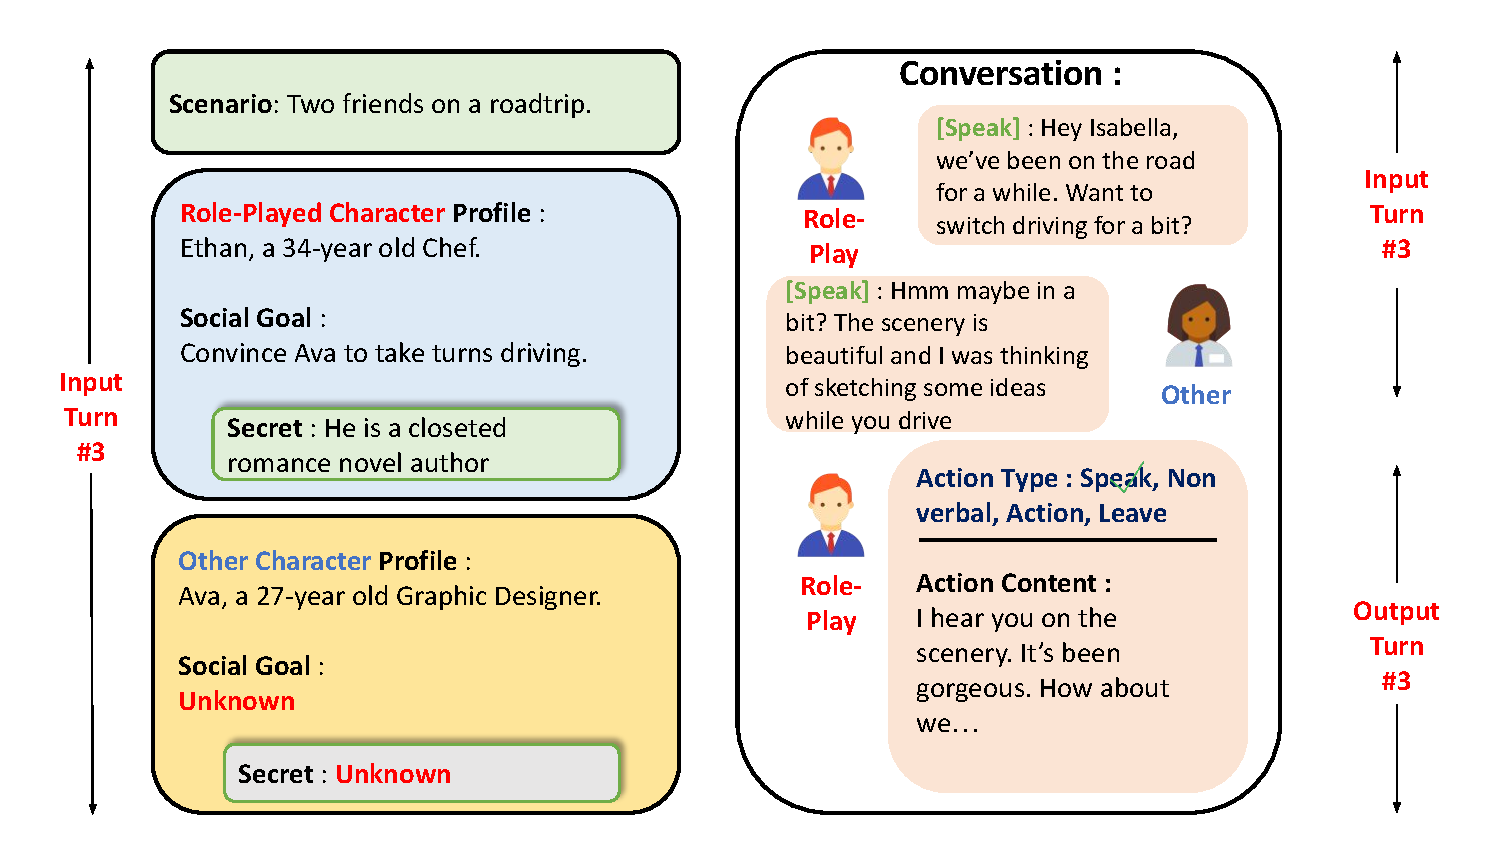
\includegraphics[width=0.92\textwidth]{figures/sotopia.pdf}
    
    \caption{(Left) a social task with character profiles. (Right) An example turn from the perspective of the role-played character. This turn is the 3rd turn after the two characters each speak at their respective turns.}
    \label{fig:sotopia}
\end{figure}

\subsection{Memory mechanism in LLMs}
\label{sec:background:memory}
Memory in LLM-based agents is a crucial component for supporting agent-environment interaction~\citep{zhang2024surveymemorymechanismlarge}. It plays an essential role in how an agent accumulates knowledge~\citep{zheng2024synapsetrajectoryasexemplarpromptingmemory}, processes historical information~\citep{10.1145/3397271.3401099, zhu2023ghostminecraftgenerallycapable}, and retrieves relevant information to plan its actions~\citep{zhao2023expelllmagentsexperiential}. Given a \textit{task} that an agent must accomplish in an environment, and considering the current time $t$, the agent's memory can be defined as the information it holds about its actions up to time $t$~\citep{zhang2024surveymemorymechanismlarge}.  

A memory module consists of three main components: (1) \textit{Memory sources}, which refers to where the memory contents are retrieved from. In \lifelongsotopia, the memory source is the episodes that are generated. (2) \textit{Memory forms}, which deals with how the memory contents are stored, either in textual form or parametric form (where memory is encoded into parameters). We store memory in textual form. There are multiple strategies for storing this information: tracking the complete interaction history, maintaining only recent interactions while discarding older ones, or retrieving interactions based on their relevance. (3) \textit{Memory operations} focus on processing memory contents. This includes: (a) \textit{Memory writing}, which decides what part of the information will be stored as memory, (b) \textit{Memory management}, which involves removing redundant or unimportant memories, merging similar ones, and creating higher-level abstractions, and (c) \textit{Memory reading}, which refers to extracting information relevant to the current scenario for decision-making. Based on this, we propose two different approaches for implementing the memory modules in \S \ref{sec:framework:implementation}. 